\documentclass[1p]{elsarticle_modified}
%\bibliographystyle{elsarticle-num}

%\usepackage[colorlinks]{hyperref}
%\usepackage{abbrmath_seonhwa} %\Abb, \Ascr, \Acal ,\Abf, \Afrak
\usepackage{amsfonts}
\usepackage{amssymb}
\usepackage{amsmath}
\usepackage{amsthm}
\usepackage{scalefnt}
\usepackage{amsbsy}
\usepackage{kotex}
\usepackage{caption}
\usepackage{subfig}
\usepackage{color}
\usepackage{graphicx}
\usepackage{xcolor} %% white, black, red, green, blue, cyan, magenta, yellow
\usepackage{float}
\usepackage{setspace}
\usepackage{hyperref}

\usepackage{tikz}
\usetikzlibrary{arrows}

\usepackage{multirow}
\usepackage{array} % fixed length table
\usepackage{hhline}

%%%%%%%%%%%%%%%%%%%%%
\makeatletter
\renewcommand*\env@matrix[1][\arraystretch]{%
	\edef\arraystretch{#1}%
	\hskip -\arraycolsep
	\let\@ifnextchar\new@ifnextchar
	\array{*\c@MaxMatrixCols c}}
\makeatother %https://tex.stackexchange.com/questions/14071/how-can-i-increase-the-line-spacing-in-a-matrix
%%%%%%%%%%%%%%%

\usepackage[normalem]{ulem}

\newcommand{\msout}[1]{\ifmmode\text{\sout{\ensuremath{#1}}}\else\sout{#1}\fi}
%SOURCE: \msout is \stkout macro in https://tex.stackexchange.com/questions/20609/strikeout-in-math-mode

\newcommand{\cancel}[1]{
	\ifmmode
	{\color{red}\msout{#1}}
	\else
	{\color{red}\sout{#1}}
	\fi
}

\newcommand{\add}[1]{
	{\color{blue}\uwave{#1}}
}

\newcommand{\replace}[2]{
	\ifmmode
	{\color{red}\msout{#1}}{\color{blue}\uwave{#2}}
	\else
	{\color{red}\sout{#1}}{\color{blue}\uwave{#2}}
	\fi
}

\newcommand{\Sol}{\mathcal{S}} %segment
\newcommand{\D}{D} %diagram
\newcommand{\A}{\mathcal{A}} %arc


%%%%%%%%%%%%%%%%%%%%%%%%%%%%%5 test

\def\sl{\operatorname{\textup{SL}}(2,\Cbb)}
\def\psl{\operatorname{\textup{PSL}}(2,\Cbb)}
\def\quan{\mkern 1mu \triangleright \mkern 1mu}

\theoremstyle{definition}
\newtheorem{thm}{Theorem}[section]
\newtheorem{prop}[thm]{Proposition}
\newtheorem{lem}[thm]{Lemma}
\newtheorem{ques}[thm]{Question}
\newtheorem{cor}[thm]{Corollary}
\newtheorem{defn}[thm]{Definition}
\newtheorem{exam}[thm]{Example}
\newtheorem{rmk}[thm]{Remark}
\newtheorem{alg}[thm]{Algorithm}

\newcommand{\I}{\sqrt{-1}}
\begin{document}

%\begin{frontmatter}
%
%\title{Boundary parabolic representations of knots up to 8 crossings}
%
%%% Group authors per affiliation:
%\author{Yunhi Cho} 
%\address{Department of Mathematics, University of Seoul, Seoul, Korea}
%\ead{yhcho@uos.ac.kr}
%
%
%\author{Seonhwa Kim} %\fnref{s_kim}}
%\address{Center for Geometry and Physics, Institute for Basic Science, Pohang, 37673, Korea}
%\ead{ryeona17@ibs.re.kr}
%
%\author{Hyuk Kim}
%\address{Department of Mathematical Sciences, Seoul National University, Seoul 08826, Korea}
%\ead{hyukkim@snu.ac.kr}
%
%\author{Seokbeom Yoon}
%\address{Department of Mathematical Sciences, Seoul National University, Seoul, 08826,  Korea}
%\ead{sbyoon15@snu.ac.kr}
%
%\begin{abstract}
%We find all boundary parabolic representation of knots up to 8 crossings.
%
%\end{abstract}
%\begin{keyword}
%    \MSC[2010] 57M25 
%\end{keyword}
%
%\end{frontmatter}

%\linenumbers
%\tableofcontents
%
\newcommand\colored[1]{\textcolor{white}{\rule[-0.35ex]{0.8em}{1.4ex}}\kern-0.8em\color{red} #1}%
%\newcommand\colored[1]{\textcolor{white}{ #1}\kern-2.17ex	\textcolor{white}{ #1}\kern-1.81ex	\textcolor{white}{ #1}\kern-2.15ex\color{red}#1	}

{\Large $\underline{12a_{0253}~(K12a_{0253})}$}

\setlength{\tabcolsep}{10pt}
\renewcommand{\arraystretch}{1.6}
\vspace{1cm}\begin{tabular}{m{100pt}>{\centering\arraybackslash}m{274pt}}
\multirow{5}{120pt}{
	\centering
	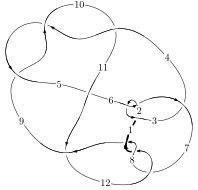
\includegraphics[width=112pt]{../../../GIT/diagram.site/Diagrams/png/1054_12a_0253.png}\\
\ \ \ A knot diagram\footnotemark}&
\allowdisplaybreaks
\textbf{Linearized knot diagam} \\
\cline{2-2}
 &
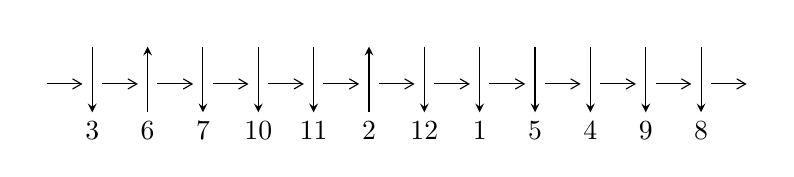
\begin{tikzpicture}[x=20pt, y=17pt]
	% nodes
	\node (C0) at (0, 0) {};
	\node (C1) at (1, 0) {};
	\node (C1U) at (1, +1) {};
	\node (C1D) at (1, -1) {3};

	\node (C2) at (2, 0) {};
	\node (C2U) at (2, +1) {};
	\node (C2D) at (2, -1) {6};

	\node (C3) at (3, 0) {};
	\node (C3U) at (3, +1) {};
	\node (C3D) at (3, -1) {7};

	\node (C4) at (4, 0) {};
	\node (C4U) at (4, +1) {};
	\node (C4D) at (4, -1) {10};

	\node (C5) at (5, 0) {};
	\node (C5U) at (5, +1) {};
	\node (C5D) at (5, -1) {11};

	\node (C6) at (6, 0) {};
	\node (C6U) at (6, +1) {};
	\node (C6D) at (6, -1) {2};

	\node (C7) at (7, 0) {};
	\node (C7U) at (7, +1) {};
	\node (C7D) at (7, -1) {12};

	\node (C8) at (8, 0) {};
	\node (C8U) at (8, +1) {};
	\node (C8D) at (8, -1) {1};

	\node (C9) at (9, 0) {};
	\node (C9U) at (9, +1) {};
	\node (C9D) at (9, -1) {5};

	\node (C10) at (10, 0) {};
	\node (C10U) at (10, +1) {};
	\node (C10D) at (10, -1) {4};

	\node (C11) at (11, 0) {};
	\node (C11U) at (11, +1) {};
	\node (C11D) at (11, -1) {9};

	\node (C12) at (12, 0) {};
	\node (C12U) at (12, +1) {};
	\node (C12D) at (12, -1) {8};
	\node (C13) at (13, 0) {};

	% arrows
	\draw[->,>={angle 60}]
	(C0) edge (C1) (C1) edge (C2) (C2) edge (C3) (C3) edge (C4) (C4) edge (C5) (C5) edge (C6) (C6) edge (C7) (C7) edge (C8) (C8) edge (C9) (C9) edge (C10) (C10) edge (C11) (C11) edge (C12) (C12) edge (C13) ;	\draw[->,>=stealth]
	(C1U) edge (C1D) (C2D) edge (C2U) (C3U) edge (C3D) (C4U) edge (C4D) (C5U) edge (C5D) (C6D) edge (C6U) (C7U) edge (C7D) (C8U) edge (C8D) (C9U) edge (C9D) (C10U) edge (C10D) (C11U) edge (C11D) (C12U) edge (C12D) ;
	\end{tikzpicture} \\
\hhline{~~} \\& 
\textbf{Solving Sequence} \\ \cline{2-2} 
 &
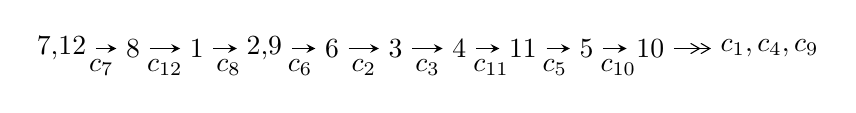
\begin{tikzpicture}[x=23pt, y=7pt]
	% node
	\node (A0) at (-1/8, 0) {7,12};
	\node (A1) at (1, 0) {8};
	\node (A2) at (2, 0) {1};
	\node (A3) at (49/16, 0) {2,9};
	\node (A4) at (33/8, 0) {6};
	\node (A5) at (41/8, 0) {3};
	\node (A6) at (49/8, 0) {4};
	\node (A7) at (57/8, 0) {11};
	\node (A8) at (65/8, 0) {5};
	\node (A9) at (73/8, 0) {10};
	\node (C1) at (1/2, -1) {$c_{7}$};
	\node (C2) at (3/2, -1) {$c_{12}$};
	\node (C3) at (5/2, -1) {$c_{8}$};
	\node (C4) at (29/8, -1) {$c_{6}$};
	\node (C5) at (37/8, -1) {$c_{2}$};
	\node (C6) at (45/8, -1) {$c_{3}$};
	\node (C7) at (53/8, -1) {$c_{11}$};
	\node (C8) at (61/8, -1) {$c_{5}$};
	\node (C9) at (69/8, -1) {$c_{10}$};
	\node (A10) at (11, 0) {$c_{1},c_{4},c_{9}$};

	% edge
	\draw[->,>=stealth]	
	(A0) edge (A1) (A1) edge (A2) (A2) edge (A3) (A3) edge (A4) (A4) edge (A5) (A5) edge (A6) (A6) edge (A7) (A7) edge (A8) (A8) edge (A9) ;
	\draw[->>,>={angle 60}]	
	(A9) edge (A10);
\end{tikzpicture} \\ 

\end{tabular} \\

\footnotetext{
The image of knot diagram is generated by the software ``\textbf{Draw programme}" developed by Andrew Bartholomew(\url{http://www.layer8.co.uk/maths/draw/index.htm\#Running-draw}), where we modified some parts for our purpose(\url{https://github.com/CATsTAILs/LinksPainter}).
}\phantom \\ \newline 
\centering \textbf{Ideals for irreducible components\footnotemark of $X_{\text{par}}$} 
 
\begin{align*}
I^u_{1}&=\langle 
9.24517\times10^{57} u^{85}-1.54464\times10^{58} u^{84}+\cdots+1.11523\times10^{58} b+1.15745\times10^{57},\\
\phantom{I^u_{1}}&\phantom{= \langle  }1.50534\times10^{56} u^{85}+3.04581\times10^{58} u^{84}+\cdots+3.34570\times10^{58} a+5.43441\times10^{59},\;u^{86}-3 u^{85}+\cdots-34 u-3\rangle \\
I^u_{2}&=\langle 
-2 a^3+a^2+3 b-2 a+12,\;a^4-2 a^3+a^2-6 a+9,\;u+1\rangle \\
I^u_{3}&=\langle 
b- a-1,\;a^2+a+1,\;u-1\rangle \\
\\
\end{align*}
\raggedright * 3 irreducible components of $\dim_{\mathbb{C}}=0$, with total 92 representations.\\
\footnotetext{All coefficients of polynomials are rational numbers. But the coefficients are sometimes approximated in decimal forms when there is not enough margin.}
\newpage
\renewcommand{\arraystretch}{1}
\centering \section*{I. $I^u_{1}= \langle 9.25\times10^{57} u^{85}-1.54\times10^{58} u^{84}+\cdots+1.12\times10^{58} b+1.16\times10^{57},\;1.51\times10^{56} u^{85}+3.05\times10^{58} u^{84}+\cdots+3.35\times10^{58} a+5.43\times10^{59},\;u^{86}-3 u^{85}+\cdots-34 u-3 \rangle$}
\flushleft \textbf{(i) Arc colorings}\\
\begin{tabular}{m{7pt} m{180pt} m{7pt} m{180pt} }
\flushright $a_{7}=$&$\begin{pmatrix}1\\0\end{pmatrix}$ \\
\flushright $a_{12}=$&$\begin{pmatrix}0\\u\end{pmatrix}$ \\
\flushright $a_{8}=$&$\begin{pmatrix}1\\u^2\end{pmatrix}$ \\
\flushright $a_{1}=$&$\begin{pmatrix}- u\\- u^3+u\end{pmatrix}$ \\
\flushright $a_{2}=$&$\begin{pmatrix}-0.00449933 u^{85}-0.910366 u^{84}+\cdots-141.366 u-16.2430\\-0.828990 u^{85}+1.38504 u^{84}+\cdots-11.9263 u-0.103785\end{pmatrix}$ \\
\flushright $a_{9}=$&$\begin{pmatrix}- u^2+1\\- u^4+2 u^2\end{pmatrix}$ \\
\flushright $a_{6}=$&$\begin{pmatrix}-0.837224 u^{85}+0.0804651 u^{84}+\cdots-130.221 u-7.83724\\-3.79661 u^{85}+6.58342 u^{84}+\cdots-86.4919 u-6.76326\end{pmatrix}$ \\
\flushright $a_{3}=$&$\begin{pmatrix}0.176785 u^{85}-1.53222 u^{84}+\cdots-115.444 u-7.32994\\-3.77989 u^{85}+6.61134 u^{84}+\cdots-69.8360 u-5.51727\end{pmatrix}$ \\
\flushright $a_{4}=$&$\begin{pmatrix}3.95667 u^{85}-8.14357 u^{84}+\cdots-45.6076 u-1.81266\\-3.77989 u^{85}+6.61134 u^{84}+\cdots-69.8360 u-5.51727\end{pmatrix}$ \\
\flushright $a_{11}=$&$\begin{pmatrix}u^5-2 u^3+u\\u^7-3 u^5+2 u^3+u\end{pmatrix}$ \\
\flushright $a_{5}=$&$\begin{pmatrix}0.170469 u^{85}-1.72112 u^{84}+\cdots-100.160 u-5.09925\\-5.50900 u^{85}+9.39416 u^{84}+\cdots-126.089 u-9.76030\end{pmatrix}$ \\
\flushright $a_{10}=$&$\begin{pmatrix}0.0483546 u^{85}+0.0549293 u^{84}+\cdots+153.570 u+22.9187\\-2.19185 u^{85}+4.26494 u^{84}+\cdots-65.2290 u-7.04254\end{pmatrix}$\\&\end{tabular}
\flushleft \textbf{(ii) Obstruction class $= -1$}\\~\\
\flushleft \textbf{(iii) Cusp Shapes $= 10.4324 u^{85}-19.4232 u^{84}+\cdots+153.225 u+9.09895$}\\~\\
\newpage\renewcommand{\arraystretch}{1}
\flushleft \textbf{(iv) u-Polynomials at the component}\newline \\
\begin{tabular}{m{50pt}|m{274pt}}
Crossings & \hspace{64pt}u-Polynomials at each crossing \\
\hline $$\begin{aligned}c_{1}\end{aligned}$$&$\begin{aligned}
&u^{86}+40 u^{85}+\cdots-49 u+9
\end{aligned}$\\
\hline $$\begin{aligned}c_{2},c_{6}\end{aligned}$$&$\begin{aligned}
&u^{86}-2 u^{85}+\cdots-5 u+3
\end{aligned}$\\
\hline $$\begin{aligned}c_{3}\end{aligned}$$&$\begin{aligned}
&u^{86}+2 u^{85}+\cdots+6103 u+867
\end{aligned}$\\
\hline $$\begin{aligned}c_{4},c_{9},c_{10}\end{aligned}$$&$\begin{aligned}
&u^{86}- u^{85}+\cdots+12 u^2-4
\end{aligned}$\\
\hline $$\begin{aligned}c_{5}\end{aligned}$$&$\begin{aligned}
&u^{86}+u^{85}+\cdots-10416 u-3764
\end{aligned}$\\
\hline $$\begin{aligned}c_{7},c_{8},c_{12}\end{aligned}$$&$\begin{aligned}
&u^{86}+3 u^{85}+\cdots+34 u-3
\end{aligned}$\\
\hline $$\begin{aligned}c_{11}\end{aligned}$$&$\begin{aligned}
&u^{86}-15 u^{85}+\cdots-39168 u+2304
\end{aligned}$\\
\hline
\end{tabular}\\~\\
\newpage\renewcommand{\arraystretch}{1}
\flushleft \textbf{(v) Riley Polynomials at the component}\newline \\
\begin{tabular}{m{50pt}|m{274pt}}
Crossings & \hspace{64pt}Riley Polynomials at each crossing \\
\hline $$\begin{aligned}c_{1}\end{aligned}$$&$\begin{aligned}
&y^{86}+16 y^{85}+\cdots-6973 y+81
\end{aligned}$\\
\hline $$\begin{aligned}c_{2},c_{6}\end{aligned}$$&$\begin{aligned}
&y^{86}+40 y^{85}+\cdots-49 y+9
\end{aligned}$\\
\hline $$\begin{aligned}c_{3}\end{aligned}$$&$\begin{aligned}
&y^{86}-8 y^{85}+\cdots-38342497 y+751689
\end{aligned}$\\
\hline $$\begin{aligned}c_{4},c_{9},c_{10}\end{aligned}$$&$\begin{aligned}
&y^{86}+81 y^{85}+\cdots-96 y+16
\end{aligned}$\\
\hline $$\begin{aligned}c_{5}\end{aligned}$$&$\begin{aligned}
&y^{86}+21 y^{85}+\cdots+479022176 y+14167696
\end{aligned}$\\
\hline $$\begin{aligned}c_{7},c_{8},c_{12}\end{aligned}$$&$\begin{aligned}
&y^{86}-73 y^{85}+\cdots-22 y+9
\end{aligned}$\\
\hline $$\begin{aligned}c_{11}\end{aligned}$$&$\begin{aligned}
&y^{86}+41 y^{85}+\cdots-33914880 y+5308416
\end{aligned}$\\
\hline
\end{tabular}\\~\\
\newpage\flushleft \textbf{(vi) Complex Volumes and Cusp Shapes}
$$\begin{array}{c|c|c}  
\text{Solutions to }I^u_{1}& \I (\text{vol} + \sqrt{-1}CS) & \text{Cusp shape}\\
 \hline 
\begin{aligned}
u &= -0.937490 + 0.430300 I \\
a &= \phantom{-}1.00429 - 1.14454 I \\
b &= -0.241775 - 1.011130 I\end{aligned}
 & \phantom{-}1.144470 + 0.306681 I & \phantom{-0.000000 } 0 \\ \hline\begin{aligned}
u &= -0.937490 - 0.430300 I \\
a &= \phantom{-}1.00429 + 1.14454 I \\
b &= -0.241775 + 1.011130 I\end{aligned}
 & \phantom{-}1.144470 - 0.306681 I & \phantom{-0.000000 } 0 \\ \hline\begin{aligned}
u &= \phantom{-}1.005680 + 0.408323 I \\
a &= -0.191946 + 0.749339 I \\
b &= \phantom{-}0.532327 + 1.041940 I\end{aligned}
 & -1.99634 + 3.50206 I & \phantom{-0.000000 } 0 \\ \hline\begin{aligned}
u &= \phantom{-}1.005680 - 0.408323 I \\
a &= -0.191946 - 0.749339 I \\
b &= \phantom{-}0.532327 - 1.041940 I\end{aligned}
 & -1.99634 - 3.50206 I & \phantom{-0.000000 } 0 \\ \hline\begin{aligned}
u &= -0.164209 + 0.884531 I \\
a &= \phantom{-}1.55407 - 0.50527 I \\
b &= -0.596084 - 1.103410 I\end{aligned}
 & \phantom{-}6.24183 + 11.34140 I & \phantom{-0.000000 } 0 \\ \hline\begin{aligned}
u &= -0.164209 - 0.884531 I \\
a &= \phantom{-}1.55407 + 0.50527 I \\
b &= -0.596084 + 1.103410 I\end{aligned}
 & \phantom{-}6.24183 - 11.34140 I & \phantom{-0.000000 } 0 \\ \hline\begin{aligned}
u &= -0.140641 + 0.851038 I \\
a &= \phantom{-}0.719793 - 0.554229 I \\
b &= -0.774320 + 0.412576 I\end{aligned}
 & \phantom{-}8.28971 + 6.17177 I & \phantom{-0.000000 } 0. - 3.86741 I \\ \hline\begin{aligned}
u &= -0.140641 - 0.851038 I \\
a &= \phantom{-}0.719793 + 0.554229 I \\
b &= -0.774320 - 0.412576 I\end{aligned}
 & \phantom{-}8.28971 - 6.17177 I & \phantom{-0.000000 -}0. + 3.86741 I \\ \hline\begin{aligned}
u &= \phantom{-}1.108240 + 0.304185 I \\
a &= -0.660682 - 0.518695 I \\
b &= \phantom{-}0.590338 - 0.517278 I\end{aligned}
 & -0.416671 - 0.977097 I & \phantom{-0.000000 } 0 \\ \hline\begin{aligned}
u &= \phantom{-}1.108240 - 0.304185 I \\
a &= -0.660682 + 0.518695 I \\
b &= \phantom{-}0.590338 + 0.517278 I\end{aligned}
 & -0.416671 + 0.977097 I & \phantom{-0.000000 } 0\\
 \hline 
 \end{array}$$\newpage$$\begin{array}{c|c|c}  
\text{Solutions to }I^u_{1}& \I (\text{vol} + \sqrt{-1}CS) & \text{Cusp shape}\\
 \hline 
\begin{aligned}
u &= \phantom{-}0.191772 + 0.814006 I \\
a &= -1.62696 - 0.60410 I \\
b &= \phantom{-}0.575207 - 1.088420 I\end{aligned}
 & \phantom{-}0.50319 - 7.91768 I & -8.00000 + 8.55988 I \\ \hline\begin{aligned}
u &= \phantom{-}0.191772 - 0.814006 I \\
a &= -1.62696 + 0.60410 I \\
b &= \phantom{-}0.575207 + 1.088420 I\end{aligned}
 & \phantom{-}0.50319 + 7.91768 I & -8.00000 - 8.55988 I \\ \hline\begin{aligned}
u &= -0.643264 + 0.517594 I \\
a &= -0.069274 + 0.763693 I \\
b &= -0.388813 + 1.051620 I\end{aligned}
 & \phantom{-}0.126526 - 1.348510 I & -10.09845 + 0.59644 I \\ \hline\begin{aligned}
u &= -0.643264 - 0.517594 I \\
a &= -0.069274 - 0.763693 I \\
b &= -0.388813 - 1.051620 I\end{aligned}
 & \phantom{-}0.126526 + 1.348510 I & -10.09845 - 0.59644 I \\ \hline\begin{aligned}
u &= \phantom{-}0.679429 + 0.440262 I \\
a &= -1.07780 - 1.26627 I \\
b &= \phantom{-}0.378317 - 1.023720 I\end{aligned}
 & -3.03860 - 2.82315 I & -15.8960 + 4.7165 I \\ \hline\begin{aligned}
u &= \phantom{-}0.679429 - 0.440262 I \\
a &= -1.07780 + 1.26627 I \\
b &= \phantom{-}0.378317 + 1.023720 I\end{aligned}
 & -3.03860 + 2.82315 I & -15.8960 - 4.7165 I \\ \hline\begin{aligned}
u &= -0.214594 + 0.780092 I \\
a &= -0.090560 + 0.441568 I \\
b &= -0.139371 + 1.089850 I\end{aligned}
 & \phantom{-}3.33866 + 4.01408 I & -7.17137 - 3.50293 I \\ \hline\begin{aligned}
u &= -0.214594 - 0.780092 I \\
a &= -0.090560 - 0.441568 I \\
b &= -0.139371 - 1.089850 I\end{aligned}
 & \phantom{-}3.33866 - 4.01408 I & -7.17137 + 3.50293 I \\ \hline\begin{aligned}
u &= -0.515177 + 0.622214 I \\
a &= \phantom{-}1.33600 - 1.11735 I \\
b &= -0.447982 - 1.078400 I\end{aligned}
 & \phantom{-}0.52472 + 5.60317 I & -8.80517 - 7.78208 I \\ \hline\begin{aligned}
u &= -0.515177 - 0.622214 I \\
a &= \phantom{-}1.33600 + 1.11735 I \\
b &= -0.447982 + 1.078400 I\end{aligned}
 & \phantom{-}0.52472 - 5.60317 I & -8.80517 + 7.78208 I\\
 \hline 
 \end{array}$$\newpage$$\begin{array}{c|c|c}  
\text{Solutions to }I^u_{1}& \I (\text{vol} + \sqrt{-1}CS) & \text{Cusp shape}\\
 \hline 
\begin{aligned}
u &= -1.119280 + 0.428552 I \\
a &= \phantom{-}0.620787 - 0.453878 I \\
b &= -0.695633 - 0.422165 I\end{aligned}
 & \phantom{-}5.30202 - 1.57924 I & \phantom{-0.000000 } 0 \\ \hline\begin{aligned}
u &= -1.119280 - 0.428552 I \\
a &= \phantom{-}0.620787 + 0.453878 I \\
b &= -0.695633 + 0.422165 I\end{aligned}
 & \phantom{-}5.30202 + 1.57924 I & \phantom{-0.000000 } 0 \\ \hline\begin{aligned}
u &= -1.105670 + 0.488129 I \\
a &= \phantom{-}0.196535 + 0.684274 I \\
b &= -0.570013 + 1.080940 I\end{aligned}
 & \phantom{-}3.37107 - 6.46244 I & \phantom{-0.000000 } 0 \\ \hline\begin{aligned}
u &= -1.105670 - 0.488129 I \\
a &= \phantom{-}0.196535 - 0.684274 I \\
b &= -0.570013 - 1.080940 I\end{aligned}
 & \phantom{-}3.37107 + 6.46244 I & \phantom{-0.000000 } 0 \\ \hline\begin{aligned}
u &= \phantom{-}0.140406 + 0.768282 I \\
a &= -0.667609 - 0.599757 I \\
b &= \phantom{-}0.717440 + 0.412450 I\end{aligned}
 & \phantom{-}2.48759 - 2.96564 I & -4.45963 + 4.32184 I \\ \hline\begin{aligned}
u &= \phantom{-}0.140406 - 0.768282 I \\
a &= -0.667609 + 0.599757 I \\
b &= \phantom{-}0.717440 - 0.412450 I\end{aligned}
 & \phantom{-}2.48759 + 2.96564 I & -4.45963 - 4.32184 I \\ \hline\begin{aligned}
u &= -1.202960 + 0.205672 I \\
a &= \phantom{-}0.342628 + 0.698123 I \\
b &= -0.626797 + 0.954629 I\end{aligned}
 & -1.81208 - 0.80751 I & \phantom{-0.000000 } 0 \\ \hline\begin{aligned}
u &= -1.202960 - 0.205672 I \\
a &= \phantom{-}0.342628 - 0.698123 I \\
b &= -0.626797 - 0.954629 I\end{aligned}
 & -1.81208 + 0.80751 I & \phantom{-0.000000 } 0 \\ \hline\begin{aligned}
u &= -1.224330 + 0.109317 I \\
a &= \phantom{-}1.69292 - 2.80660 I \\
b &= \phantom{-}0.304875 - 0.972720 I\end{aligned}
 & \phantom{-}1.75123 - 1.09860 I & \phantom{-0.000000 } 0 \\ \hline\begin{aligned}
u &= -1.224330 - 0.109317 I \\
a &= \phantom{-}1.69292 + 2.80660 I \\
b &= \phantom{-}0.304875 + 0.972720 I\end{aligned}
 & \phantom{-}1.75123 + 1.09860 I & \phantom{-0.000000 } 0\\
 \hline 
 \end{array}$$\newpage$$\begin{array}{c|c|c}  
\text{Solutions to }I^u_{1}& \I (\text{vol} + \sqrt{-1}CS) & \text{Cusp shape}\\
 \hline 
\begin{aligned}
u &= -0.059355 + 0.763438 I \\
a &= -0.842674 - 0.752985 I \\
b &= \phantom{-}0.727407 + 0.546983 I\end{aligned}
 & \phantom{-}9.00597 + 3.45050 I & \phantom{-}0.30379 - 3.33870 I \\ \hline\begin{aligned}
u &= -0.059355 - 0.763438 I \\
a &= -0.842674 + 0.752985 I \\
b &= \phantom{-}0.727407 - 0.546983 I\end{aligned}
 & \phantom{-}9.00597 - 3.45050 I & \phantom{-}0.30379 + 3.33870 I \\ \hline\begin{aligned}
u &= -1.209790 + 0.313017 I \\
a &= \phantom{-}0.618892 + 0.832585 I \\
b &= \phantom{-}0.670549 - 0.456636 I\end{aligned}
 & \phantom{-}5.48833 + 0.44898 I & \phantom{-0.000000 } 0 \\ \hline\begin{aligned}
u &= -1.209790 - 0.313017 I \\
a &= \phantom{-}0.618892 - 0.832585 I \\
b &= \phantom{-}0.670549 + 0.456636 I\end{aligned}
 & \phantom{-}5.48833 - 0.44898 I & \phantom{-0.000000 } 0 \\ \hline\begin{aligned}
u &= \phantom{-}1.276820 + 0.021621 I \\
a &= -0.460719 - 0.637385 I \\
b &= \phantom{-}0.678388 - 0.823248 I\end{aligned}
 & \phantom{-}0.65889 - 2.60578 I & \phantom{-0.000000 } 0 \\ \hline\begin{aligned}
u &= \phantom{-}1.276820 - 0.021621 I \\
a &= -0.460719 + 0.637385 I \\
b &= \phantom{-}0.678388 + 0.823248 I\end{aligned}
 & \phantom{-}0.65889 + 2.60578 I & \phantom{-0.000000 } 0 \\ \hline\begin{aligned}
u &= -1.250950 + 0.268546 I \\
a &= \phantom{-}0.564274 - 0.541799 I \\
b &= -0.707247 - 0.625782 I\end{aligned}
 & -0.84391 + 4.29232 I & \phantom{-0.000000 } 0 \\ \hline\begin{aligned}
u &= -1.250950 - 0.268546 I \\
a &= \phantom{-}0.564274 + 0.541799 I \\
b &= -0.707247 + 0.625782 I\end{aligned}
 & -0.84391 - 4.29232 I & \phantom{-0.000000 } 0 \\ \hline\begin{aligned}
u &= -0.012356 + 0.713233 I \\
a &= -1.99890 - 0.30381 I \\
b &= \phantom{-}0.611337 - 1.024340 I\end{aligned}
 & \phantom{-}7.58994 - 1.66047 I & -1.74027 + 2.14109 I \\ \hline\begin{aligned}
u &= -0.012356 - 0.713233 I \\
a &= -1.99890 + 0.30381 I \\
b &= \phantom{-}0.611337 + 1.024340 I\end{aligned}
 & \phantom{-}7.58994 + 1.66047 I & -1.74027 - 2.14109 I\\
 \hline 
 \end{array}$$\newpage$$\begin{array}{c|c|c}  
\text{Solutions to }I^u_{1}& \I (\text{vol} + \sqrt{-1}CS) & \text{Cusp shape}\\
 \hline 
\begin{aligned}
u &= -0.140963 + 0.690414 I \\
a &= \phantom{-}1.88863 - 0.66965 I \\
b &= -0.567774 - 1.045600 I\end{aligned}
 & \phantom{-}1.27316 + 4.01440 I & -5.59358 - 2.50795 I \\ \hline\begin{aligned}
u &= -0.140963 - 0.690414 I \\
a &= \phantom{-}1.88863 + 0.66965 I \\
b &= -0.567774 + 1.045600 I\end{aligned}
 & \phantom{-}1.27316 - 4.01440 I & -5.59358 + 2.50795 I \\ \hline\begin{aligned}
u &= -1.268500 + 0.283353 I \\
a &= -1.85901 + 2.51368 I \\
b &= \phantom{-}0.564722 + 1.064450 I\end{aligned}
 & \phantom{-}3.69862 + 5.25403 I & \phantom{-0.000000 } 0 \\ \hline\begin{aligned}
u &= -1.268500 - 0.283353 I \\
a &= -1.85901 - 2.51368 I \\
b &= \phantom{-}0.564722 - 1.064450 I\end{aligned}
 & \phantom{-}3.69862 - 5.25403 I & \phantom{-0.000000 } 0 \\ \hline\begin{aligned}
u &= \phantom{-}0.285903 + 0.636287 I \\
a &= \phantom{-}0.203378 + 0.466290 I \\
b &= \phantom{-}0.211263 + 1.020930 I\end{aligned}
 & -1.89412 - 1.00150 I & -12.28501 + 3.83404 I \\ \hline\begin{aligned}
u &= \phantom{-}0.285903 - 0.636287 I \\
a &= \phantom{-}0.203378 - 0.466290 I \\
b &= \phantom{-}0.211263 - 1.020930 I\end{aligned}
 & -1.89412 + 1.00150 I & -12.28501 - 3.83404 I \\ \hline\begin{aligned}
u &= -0.032720 + 0.696278 I \\
a &= \phantom{-}0.678188 - 0.750281 I \\
b &= -0.672048 + 0.493933 I\end{aligned}
 & \phantom{-}2.90283 - 0.80168 I & -2.77950 + 3.30570 I \\ \hline\begin{aligned}
u &= -0.032720 - 0.696278 I \\
a &= \phantom{-}0.678188 + 0.750281 I \\
b &= -0.672048 - 0.493933 I\end{aligned}
 & \phantom{-}2.90283 + 0.80168 I & -2.77950 - 3.30570 I \\ \hline\begin{aligned}
u &= \phantom{-}1.281200 + 0.292712 I \\
a &= -0.307225 + 0.653899 I \\
b &= \phantom{-}0.662193 + 1.001970 I\end{aligned}
 & \phantom{-}3.56173 - 1.97670 I & \phantom{-0.000000 } 0 \\ \hline\begin{aligned}
u &= \phantom{-}1.281200 - 0.292712 I \\
a &= -0.307225 - 0.653899 I \\
b &= \phantom{-}0.662193 - 1.001970 I\end{aligned}
 & \phantom{-}3.56173 + 1.97670 I & \phantom{-0.000000 } 0\\
 \hline 
 \end{array}$$\newpage$$\begin{array}{c|c|c}  
\text{Solutions to }I^u_{1}& \I (\text{vol} + \sqrt{-1}CS) & \text{Cusp shape}\\
 \hline 
\begin{aligned}
u &= -0.475283 + 0.484878 I \\
a &= \phantom{-}0.510538 - 0.361911 I \\
b &= -0.542318 + 0.119668 I\end{aligned}
 & \phantom{-}3.06367 + 1.77620 I & -4.34056 - 4.01240 I \\ \hline\begin{aligned}
u &= -0.475283 - 0.484878 I \\
a &= \phantom{-}0.510538 + 0.361911 I \\
b &= -0.542318 - 0.119668 I\end{aligned}
 & \phantom{-}3.06367 - 1.77620 I & -4.34056 + 4.01240 I \\ \hline\begin{aligned}
u &= \phantom{-}1.299880 + 0.276010 I \\
a &= -0.542867 + 0.559023 I \\
b &= -0.717220 - 0.354248 I\end{aligned}
 & -1.25881 - 2.70593 I & \phantom{-0.000000 } 0 \\ \hline\begin{aligned}
u &= \phantom{-}1.299880 - 0.276010 I \\
a &= -0.542867 - 0.559023 I \\
b &= -0.717220 + 0.354248 I\end{aligned}
 & -1.25881 + 2.70593 I & \phantom{-0.000000 } 0 \\ \hline\begin{aligned}
u &= \phantom{-}1.304220 + 0.324168 I \\
a &= -0.546651 - 0.509287 I \\
b &= \phantom{-}0.770756 - 0.604539 I\end{aligned}
 & \phantom{-}4.74301 - 7.37621 I & \phantom{-0.000000 } 0 \\ \hline\begin{aligned}
u &= \phantom{-}1.304220 - 0.324168 I \\
a &= -0.546651 + 0.509287 I \\
b &= \phantom{-}0.770756 + 0.604539 I\end{aligned}
 & \phantom{-}4.74301 + 7.37621 I & \phantom{-0.000000 } 0 \\ \hline\begin{aligned}
u &= \phantom{-}1.352410 + 0.174405 I \\
a &= -0.81324 - 2.16272 I \\
b &= -0.249471 - 1.099780 I\end{aligned}
 & -5.55408 - 0.16925 I & \phantom{-0.000000 } 0 \\ \hline\begin{aligned}
u &= \phantom{-}1.352410 - 0.174405 I \\
a &= -0.81324 + 2.16272 I \\
b &= -0.249471 + 1.099780 I\end{aligned}
 & -5.55408 + 0.16925 I & \phantom{-0.000000 } 0 \\ \hline\begin{aligned}
u &= \phantom{-}1.352140 + 0.292186 I \\
a &= \phantom{-}1.43499 + 2.27569 I \\
b &= -0.563322 + 1.107880 I\end{aligned}
 & -3.45130 - 7.60457 I & \phantom{-0.000000 } 0 \\ \hline\begin{aligned}
u &= \phantom{-}1.352140 - 0.292186 I \\
a &= \phantom{-}1.43499 - 2.27569 I \\
b &= -0.563322 - 1.107880 I\end{aligned}
 & -3.45130 + 7.60457 I & \phantom{-0.000000 } 0\\
 \hline 
 \end{array}$$\newpage$$\begin{array}{c|c|c}  
\text{Solutions to }I^u_{1}& \I (\text{vol} + \sqrt{-1}CS) & \text{Cusp shape}\\
 \hline 
\begin{aligned}
u &= -1.38831\phantom{ +0.000000I} \\
a &= \phantom{-}0.567618\phantom{ +0.000000I} \\
b &= \phantom{-}0.720202\phantom{ +0.000000I}\end{aligned}
 & -6.55086\phantom{ +0.000000I} & \phantom{-0.000000 } 0 \\ \hline\begin{aligned}
u &= -1.351850 + 0.324366 I \\
a &= \phantom{-}0.391496 + 0.542908 I \\
b &= \phantom{-}0.791439 - 0.364830 I\end{aligned}
 & -2.21861 + 6.91647 I & \phantom{-0.000000 } 0 \\ \hline\begin{aligned}
u &= -1.351850 - 0.324366 I \\
a &= \phantom{-}0.391496 - 0.542908 I \\
b &= \phantom{-}0.791439 + 0.364830 I\end{aligned}
 & -2.21861 - 6.91647 I & \phantom{-0.000000 } 0 \\ \hline\begin{aligned}
u &= \phantom{-}1.393980 + 0.099240 I \\
a &= -0.540745 + 0.161854 I \\
b &= -0.738441 - 0.118627 I\end{aligned}
 & -2.87844 - 3.59222 I & \phantom{-0.000000 } 0 \\ \hline\begin{aligned}
u &= \phantom{-}1.393980 - 0.099240 I \\
a &= -0.540745 - 0.161854 I \\
b &= -0.738441 + 0.118627 I\end{aligned}
 & -2.87844 + 3.59222 I & \phantom{-0.000000 } 0 \\ \hline\begin{aligned}
u &= -1.381300 + 0.261910 I \\
a &= \phantom{-}0.76597 - 1.83243 I \\
b &= \phantom{-}0.185250 - 1.144530 I\end{aligned}
 & -7.11430 + 4.28554 I & \phantom{-0.000000 } 0 \\ \hline\begin{aligned}
u &= -1.381300 - 0.261910 I \\
a &= \phantom{-}0.76597 + 1.83243 I \\
b &= \phantom{-}0.185250 + 1.144530 I\end{aligned}
 & -7.11430 - 4.28554 I & \phantom{-0.000000 } 0 \\ \hline\begin{aligned}
u &= \phantom{-}1.361770 + 0.368227 I \\
a &= -0.313580 + 0.571371 I \\
b &= -0.822713 - 0.393707 I\end{aligned}
 & \phantom{-}3.55461 - 10.55500 I & \phantom{-0.000000 } 0 \\ \hline\begin{aligned}
u &= \phantom{-}1.361770 - 0.368227 I \\
a &= -0.313580 - 0.571371 I \\
b &= -0.822713 + 0.393707 I\end{aligned}
 & \phantom{-}3.55461 + 10.55500 I & \phantom{-0.000000 } 0 \\ \hline\begin{aligned}
u &= \phantom{-}1.38140 + 0.32368 I \\
a &= -0.76839 - 1.67329 I \\
b &= -0.139012 - 1.165260 I\end{aligned}
 & -1.70286 - 8.00114 I & \phantom{-0.000000 } 0\\
 \hline 
 \end{array}$$\newpage$$\begin{array}{c|c|c}  
\text{Solutions to }I^u_{1}& \I (\text{vol} + \sqrt{-1}CS) & \text{Cusp shape}\\
 \hline 
\begin{aligned}
u &= \phantom{-}1.38140 - 0.32368 I \\
a &= -0.76839 + 1.67329 I \\
b &= -0.139012 + 1.165260 I\end{aligned}
 & -1.70286 + 8.00114 I & \phantom{-0.000000 } 0 \\ \hline\begin{aligned}
u &= -1.38065 + 0.34200 I \\
a &= -1.41854 + 2.02252 I \\
b &= \phantom{-}0.587418 + 1.124720 I\end{aligned}
 & -4.46950 + 12.08680 I & \phantom{-0.000000 } 0 \\ \hline\begin{aligned}
u &= -1.38065 - 0.34200 I \\
a &= -1.41854 - 2.02252 I \\
b &= \phantom{-}0.587418 - 1.124720 I\end{aligned}
 & -4.46950 - 12.08680 I & \phantom{-0.000000 } 0 \\ \hline\begin{aligned}
u &= \phantom{-}1.43042 + 0.03954 I \\
a &= -0.16221 - 2.40323 I \\
b &= -0.360833 - 1.146350 I\end{aligned}
 & -6.62289 + 0.05087 I & \phantom{-0.000000 } 0 \\ \hline\begin{aligned}
u &= \phantom{-}1.43042 - 0.03954 I \\
a &= -0.16221 + 2.40323 I \\
b &= -0.360833 + 1.146350 I\end{aligned}
 & -6.62289 - 0.05087 I & \phantom{-0.000000 } 0 \\ \hline\begin{aligned}
u &= \phantom{-}1.38019 + 0.38195 I \\
a &= \phantom{-}1.47204 + 1.87953 I \\
b &= -0.607318 + 1.125960 I\end{aligned}
 & \phantom{-}1.3661 - 15.8872 I & \phantom{-0.000000 } 0 \\ \hline\begin{aligned}
u &= \phantom{-}1.38019 - 0.38195 I \\
a &= \phantom{-}1.47204 - 1.87953 I \\
b &= -0.607318 - 1.125960 I\end{aligned}
 & \phantom{-}1.3661 + 15.8872 I & \phantom{-0.000000 } 0 \\ \hline\begin{aligned}
u &= -1.44057 + 0.05057 I \\
a &= -0.23575 + 2.46811 I \\
b &= \phantom{-}0.421098 + 1.150570 I\end{aligned}
 & -9.88134 + 4.04361 I & \phantom{-0.000000 } 0 \\ \hline\begin{aligned}
u &= -1.44057 - 0.05057 I \\
a &= -0.23575 - 2.46811 I \\
b &= \phantom{-}0.421098 - 1.150570 I\end{aligned}
 & -9.88134 - 4.04361 I & \phantom{-0.000000 } 0 \\ \hline\begin{aligned}
u &= \phantom{-}1.44058 + 0.13086 I \\
a &= \phantom{-}0.59079 + 2.42841 I \\
b &= -0.470411 + 1.150770 I\end{aligned}
 & -5.89285 - 8.01676 I & \phantom{-0.000000 } 0\\
 \hline 
 \end{array}$$\newpage$$\begin{array}{c|c|c}  
\text{Solutions to }I^u_{1}& \I (\text{vol} + \sqrt{-1}CS) & \text{Cusp shape}\\
 \hline 
\begin{aligned}
u &= \phantom{-}1.44058 - 0.13086 I \\
a &= \phantom{-}0.59079 - 2.42841 I \\
b &= -0.470411 - 1.150770 I\end{aligned}
 & -5.89285 + 8.01676 I & \phantom{-0.000000 } 0 \\ \hline\begin{aligned}
u &= \phantom{-}0.455616\phantom{ +0.000000I} \\
a &= -0.438747\phantom{ +0.000000I} \\
b &= \phantom{-}0.323601\phantom{ +0.000000I}\end{aligned}
 & -0.724667\phantom{ +0.000000I} & -13.5020\phantom{ +0.000000I} \\ \hline\begin{aligned}
u &= -0.299519 + 0.225484 I \\
a &= -1.06879 + 1.18717 I \\
b &= -0.385808 + 0.901420 I\end{aligned}
 & -0.52400 - 1.62426 I & -4.72668 + 3.34789 I \\ \hline\begin{aligned}
u &= -0.299519 - 0.225484 I \\
a &= -1.06879 - 1.18717 I \\
b &= -0.385808 - 0.901420 I\end{aligned}
 & -0.52400 + 1.62426 I & -4.72668 - 3.34789 I \\ \hline\begin{aligned}
u &= -0.128640 + 0.138655 I \\
a &= -0.21986 - 5.36593 I \\
b &= \phantom{-}0.522501 + 0.812392 I\end{aligned}
 & \phantom{-}4.95984 + 2.14799 I & \phantom{-}0.37118 - 3.75545 I \\ \hline\begin{aligned}
u &= -0.128640 - 0.138655 I \\
a &= -0.21986 + 5.36593 I \\
b &= \phantom{-}0.522501 - 0.812392 I\end{aligned}
 & \phantom{-}4.95984 - 2.14799 I & \phantom{-}0.37118 + 3.75545 I\\
 \hline 
 \end{array}$$\newpage\newpage\renewcommand{\arraystretch}{1}
\centering \section*{II. $I^u_{2}= \langle -2 a^3+a^2+3 b-2 a+12,\;a^4-2 a^3+a^2-6 a+9,\;u+1 \rangle$}
\flushleft \textbf{(i) Arc colorings}\\
\begin{tabular}{m{7pt} m{180pt} m{7pt} m{180pt} }
\flushright $a_{7}=$&$\begin{pmatrix}1\\0\end{pmatrix}$ \\
\flushright $a_{12}=$&$\begin{pmatrix}0\\-1\end{pmatrix}$ \\
\flushright $a_{8}=$&$\begin{pmatrix}1\\1\end{pmatrix}$ \\
\flushright $a_{1}=$&$\begin{pmatrix}1\\0\end{pmatrix}$ \\
\flushright $a_{2}=$&$\begin{pmatrix}a\\\frac{2}{3} a^3-\frac{1}{3} a^2+\frac{2}{3} a-4\end{pmatrix}$ \\
\flushright $a_{9}=$&$\begin{pmatrix}0\\1\end{pmatrix}$ \\
\flushright $a_{6}=$&$\begin{pmatrix}a^3-5\\-\frac{2}{3} a^3+\frac{1}{3} a^2-\frac{2}{3} a+3\end{pmatrix}$ \\
\flushright $a_{3}=$&$\begin{pmatrix}-\frac{1}{3} a^3-\frac{1}{3} a^2+\frac{2}{3} a+2\\\frac{2}{3} a^3-\frac{1}{3} a^2+\frac{2}{3} a-3\end{pmatrix}$ \\
\flushright $a_{4}=$&$\begin{pmatrix}- a^3+5\\\frac{2}{3} a^3-\frac{1}{3} a^2+\frac{2}{3} a-3\end{pmatrix}$ \\
\flushright $a_{11}=$&$\begin{pmatrix}0\\-1\end{pmatrix}$ \\
\flushright $a_{5}=$&$\begin{pmatrix}a^3-5\\-\frac{5}{3} a^3+\frac{1}{3} a^2-\frac{2}{3} a+8\end{pmatrix}$ \\
\flushright $a_{10}=$&$\begin{pmatrix}2\\\frac{2}{3} a^3-\frac{1}{3} a^2-\frac{1}{3} a-4\end{pmatrix}$\\&\end{tabular}
\flushleft \textbf{(ii) Obstruction class $= 1$}\\~\\
\flushleft \textbf{(iii) Cusp Shapes $= \frac{8}{3} a^3-\frac{4}{3} a^2+\frac{8}{3} a-20$}\\~\\
\newpage\renewcommand{\arraystretch}{1}
\flushleft \textbf{(iv) u-Polynomials at the component}\newline \\
\begin{tabular}{m{50pt}|m{274pt}}
Crossings & \hspace{64pt}u-Polynomials at each crossing \\
\hline $$\begin{aligned}c_{1},c_{2}\end{aligned}$$&$\begin{aligned}
&(u^2- u+1)^2
\end{aligned}$\\
\hline $$\begin{aligned}c_{3},c_{6}\end{aligned}$$&$\begin{aligned}
&(u^2+u+1)^2
\end{aligned}$\\
\hline $$\begin{aligned}c_{4},c_{5},c_{9}\\c_{10}\end{aligned}$$&$\begin{aligned}
&(u^2+2)^2
\end{aligned}$\\
\hline $$\begin{aligned}c_{7},c_{8}\end{aligned}$$&$\begin{aligned}
&(u+1)^4
\end{aligned}$\\
\hline $$\begin{aligned}c_{11}\end{aligned}$$&$\begin{aligned}
&u^4
\end{aligned}$\\
\hline $$\begin{aligned}c_{12}\end{aligned}$$&$\begin{aligned}
&(u-1)^4
\end{aligned}$\\
\hline
\end{tabular}\\~\\
\newpage\renewcommand{\arraystretch}{1}
\flushleft \textbf{(v) Riley Polynomials at the component}\newline \\
\begin{tabular}{m{50pt}|m{274pt}}
Crossings & \hspace{64pt}Riley Polynomials at each crossing \\
\hline $$\begin{aligned}c_{1},c_{2},c_{3}\\c_{6}\end{aligned}$$&$\begin{aligned}
&(y^2+y+1)^2
\end{aligned}$\\
\hline $$\begin{aligned}c_{4},c_{5},c_{9}\\c_{10}\end{aligned}$$&$\begin{aligned}
&(y+2)^4
\end{aligned}$\\
\hline $$\begin{aligned}c_{7},c_{8},c_{12}\end{aligned}$$&$\begin{aligned}
&(y-1)^4
\end{aligned}$\\
\hline $$\begin{aligned}c_{11}\end{aligned}$$&$\begin{aligned}
&y^4
\end{aligned}$\\
\hline
\end{tabular}\\~\\
\newpage\flushleft \textbf{(vi) Complex Volumes and Cusp Shapes}
$$\begin{array}{c|c|c}  
\text{Solutions to }I^u_{2}& \I (\text{vol} + \sqrt{-1}CS) & \text{Cusp shape}\\
 \hline 
\begin{aligned}
u &= -1.00000\phantom{ +0.000000I} \\
a &= \phantom{-}1.72474 + 0.15892 I \\
b &= -0.500000 + 0.866025 I\end{aligned}
 & \phantom{-}3.28987 - 2.02988 I & -6.00000 + 3.46410 I \\ \hline\begin{aligned}
u &= -1.00000\phantom{ +0.000000I} \\
a &= \phantom{-}1.72474 - 0.15892 I \\
b &= -0.500000 - 0.866025 I\end{aligned}
 & \phantom{-}3.28987 + 2.02988 I & -6.00000 - 3.46410 I \\ \hline\begin{aligned}
u &= -1.00000\phantom{ +0.000000I} \\
a &= -0.72474 + 1.57313 I \\
b &= -0.500000 + 0.866025 I\end{aligned}
 & \phantom{-}3.28987 - 2.02988 I & -6.00000 + 3.46410 I \\ \hline\begin{aligned}
u &= -1.00000\phantom{ +0.000000I} \\
a &= -0.72474 - 1.57313 I \\
b &= -0.500000 - 0.866025 I\end{aligned}
 & \phantom{-}3.28987 + 2.02988 I & -6.00000 - 3.46410 I\\
 \hline 
 \end{array}$$\newpage\newpage\renewcommand{\arraystretch}{1}
\centering \section*{III. $I^u_{3}= \langle b- a-1,\;a^2+a+1,\;u-1 \rangle$}
\flushleft \textbf{(i) Arc colorings}\\
\begin{tabular}{m{7pt} m{180pt} m{7pt} m{180pt} }
\flushright $a_{7}=$&$\begin{pmatrix}1\\0\end{pmatrix}$ \\
\flushright $a_{12}=$&$\begin{pmatrix}0\\1\end{pmatrix}$ \\
\flushright $a_{8}=$&$\begin{pmatrix}1\\1\end{pmatrix}$ \\
\flushright $a_{1}=$&$\begin{pmatrix}-1\\0\end{pmatrix}$ \\
\flushright $a_{2}=$&$\begin{pmatrix}a\\a+1\end{pmatrix}$ \\
\flushright $a_{9}=$&$\begin{pmatrix}0\\1\end{pmatrix}$ \\
\flushright $a_{6}=$&$\begin{pmatrix}0\\a\end{pmatrix}$ \\
\flushright $a_{3}=$&$\begin{pmatrix}a\\a\end{pmatrix}$ \\
\flushright $a_{4}=$&$\begin{pmatrix}0\\a\end{pmatrix}$ \\
\flushright $a_{11}=$&$\begin{pmatrix}0\\1\end{pmatrix}$ \\
\flushright $a_{5}=$&$\begin{pmatrix}0\\a\end{pmatrix}$ \\
\flushright $a_{10}=$&$\begin{pmatrix}0\\1\end{pmatrix}$\\&\end{tabular}
\flushleft \textbf{(ii) Obstruction class $= 1$}\\~\\
\flushleft \textbf{(iii) Cusp Shapes $= -4 a-14$}\\~\\
\newpage\renewcommand{\arraystretch}{1}
\flushleft \textbf{(iv) u-Polynomials at the component}\newline \\
\begin{tabular}{m{50pt}|m{274pt}}
Crossings & \hspace{64pt}u-Polynomials at each crossing \\
\hline $$\begin{aligned}c_{1},c_{3},c_{6}\end{aligned}$$&$\begin{aligned}
&u^2- u+1
\end{aligned}$\\
\hline $$\begin{aligned}c_{2}\end{aligned}$$&$\begin{aligned}
&u^2+u+1
\end{aligned}$\\
\hline $$\begin{aligned}c_{4},c_{5},c_{9}\\c_{10},c_{11}\end{aligned}$$&$\begin{aligned}
&u^2
\end{aligned}$\\
\hline $$\begin{aligned}c_{7},c_{8}\end{aligned}$$&$\begin{aligned}
&(u-1)^2
\end{aligned}$\\
\hline $$\begin{aligned}c_{12}\end{aligned}$$&$\begin{aligned}
&(u+1)^2
\end{aligned}$\\
\hline
\end{tabular}\\~\\
\newpage\renewcommand{\arraystretch}{1}
\flushleft \textbf{(v) Riley Polynomials at the component}\newline \\
\begin{tabular}{m{50pt}|m{274pt}}
Crossings & \hspace{64pt}Riley Polynomials at each crossing \\
\hline $$\begin{aligned}c_{1},c_{2},c_{3}\\c_{6}\end{aligned}$$&$\begin{aligned}
&y^2+y+1
\end{aligned}$\\
\hline $$\begin{aligned}c_{4},c_{5},c_{9}\\c_{10},c_{11}\end{aligned}$$&$\begin{aligned}
&y^2
\end{aligned}$\\
\hline $$\begin{aligned}c_{7},c_{8},c_{12}\end{aligned}$$&$\begin{aligned}
&(y-1)^2
\end{aligned}$\\
\hline
\end{tabular}\\~\\
\newpage\flushleft \textbf{(vi) Complex Volumes and Cusp Shapes}
$$\begin{array}{c|c|c}  
\text{Solutions to }I^u_{3}& \I (\text{vol} + \sqrt{-1}CS) & \text{Cusp shape}\\
 \hline 
\begin{aligned}
u &= \phantom{-}1.00000\phantom{ +0.000000I} \\
a &= -0.500000 + 0.866025 I \\
b &= \phantom{-}0.500000 + 0.866025 I\end{aligned}
 & -1.64493 + 2.02988 I & -12.00000 - 3.46410 I \\ \hline\begin{aligned}
u &= \phantom{-}1.00000\phantom{ +0.000000I} \\
a &= -0.500000 - 0.866025 I \\
b &= \phantom{-}0.500000 - 0.866025 I\end{aligned}
 & -1.64493 - 2.02988 I & -12.00000 + 3.46410 I\\
 \hline 
 \end{array}$$\newpage
\newpage\renewcommand{\arraystretch}{1}
\centering \section*{ IV. u-Polynomials}
\begin{tabular}{m{50pt}|m{274pt}}
Crossings & \hspace{64pt}u-Polynomials at each crossing \\
\hline $$\begin{aligned}c_{1}\end{aligned}$$&$\begin{aligned}
&((u^2- u+1)^3)(u^{86}+40 u^{85}+\cdots-49 u+9)
\end{aligned}$\\
\hline $$\begin{aligned}c_{2}\end{aligned}$$&$\begin{aligned}
&((u^2- u+1)^2)(u^2+u+1)(u^{86}-2 u^{85}+\cdots-5 u+3)
\end{aligned}$\\
\hline $$\begin{aligned}c_{3}\end{aligned}$$&$\begin{aligned}
&(u^2- u+1)(u^2+u+1)^2(u^{86}+2 u^{85}+\cdots+6103 u+867)
\end{aligned}$\\
\hline $$\begin{aligned}c_{4},c_{9},c_{10}\end{aligned}$$&$\begin{aligned}
&u^2(u^2+2)^2(u^{86}- u^{85}+\cdots+12 u^2-4)
\end{aligned}$\\
\hline $$\begin{aligned}c_{5}\end{aligned}$$&$\begin{aligned}
&u^2(u^2+2)^2(u^{86}+u^{85}+\cdots-10416 u-3764)
\end{aligned}$\\
\hline $$\begin{aligned}c_{6}\end{aligned}$$&$\begin{aligned}
&(u^2- u+1)(u^2+u+1)^2(u^{86}-2 u^{85}+\cdots-5 u+3)
\end{aligned}$\\
\hline $$\begin{aligned}c_{7},c_{8}\end{aligned}$$&$\begin{aligned}
&((u-1)^2)(u+1)^4(u^{86}+3 u^{85}+\cdots+34 u-3)
\end{aligned}$\\
\hline $$\begin{aligned}c_{11}\end{aligned}$$&$\begin{aligned}
&u^6(u^{86}-15 u^{85}+\cdots-39168 u+2304)
\end{aligned}$\\
\hline $$\begin{aligned}c_{12}\end{aligned}$$&$\begin{aligned}
&((u-1)^4)(u+1)^2(u^{86}+3 u^{85}+\cdots+34 u-3)
\end{aligned}$\\
\hline
\end{tabular}\newpage\renewcommand{\arraystretch}{1}
\centering \section*{ V. Riley Polynomials}
\begin{tabular}{m{50pt}|m{274pt}}
Crossings & \hspace{64pt}Riley Polynomials at each crossing \\
\hline $$\begin{aligned}c_{1}\end{aligned}$$&$\begin{aligned}
&((y^2+y+1)^3)(y^{86}+16 y^{85}+\cdots-6973 y+81)
\end{aligned}$\\
\hline $$\begin{aligned}c_{2},c_{6}\end{aligned}$$&$\begin{aligned}
&((y^2+y+1)^3)(y^{86}+40 y^{85}+\cdots-49 y+9)
\end{aligned}$\\
\hline $$\begin{aligned}c_{3}\end{aligned}$$&$\begin{aligned}
&((y^2+y+1)^3)(y^{86}-8 y^{85}+\cdots-3.83425\times10^{7} y+751689)
\end{aligned}$\\
\hline $$\begin{aligned}c_{4},c_{9},c_{10}\end{aligned}$$&$\begin{aligned}
&y^2(y+2)^4(y^{86}+81 y^{85}+\cdots-96 y+16)
\end{aligned}$\\
\hline $$\begin{aligned}c_{5}\end{aligned}$$&$\begin{aligned}
&y^2(y+2)^4(y^{86}+21 y^{85}+\cdots+4.79022\times10^{8} y+1.41677\times10^{7})
\end{aligned}$\\
\hline $$\begin{aligned}c_{7},c_{8},c_{12}\end{aligned}$$&$\begin{aligned}
&((y-1)^6)(y^{86}-73 y^{85}+\cdots-22 y+9)
\end{aligned}$\\
\hline $$\begin{aligned}c_{11}\end{aligned}$$&$\begin{aligned}
&y^6(y^{86}+41 y^{85}+\cdots-3.39149\times10^{7} y+5308416)
\end{aligned}$\\
\hline
\end{tabular}
\vskip 2pc
\end{document}